\chapter{System Design}

\section{System Architecture}
BuildScan~3D uses a three-tier client-server architecture:

\begin{enumerate}
    \item \textbf{Client tier}: Android application (ARCore capture, upload, progress display).
    \item \textbf{Server tier}: FastAPI backend (job management, pipeline orchestration, RunPod dispatch).
    \item \textbf{Compute tier}: GPU processing (local or RunPod on-demand pod running COLMAP + Nerfstudio).
\end{enumerate}

The data flow is strictly sequential: Capture $\rightarrow$ Upload $\rightarrow$ Process $\rightarrow$ Download. The server acts as an orchestrator that manages the GPU lifecycle and provides progress updates to the client via polling. Figure~\ref{fig:architecture} shows the components of each tier and how they talk to each other. The server runs in one of four processing modes set through \texttt{/config}: \texttt{dry\_run} (the default: uploads are saved, nothing is processed), \texttt{local}, \texttt{runpod} and \texttt{remote} (a fixed GPU host over SSH).

\begin{figure}[htbp]
\centering
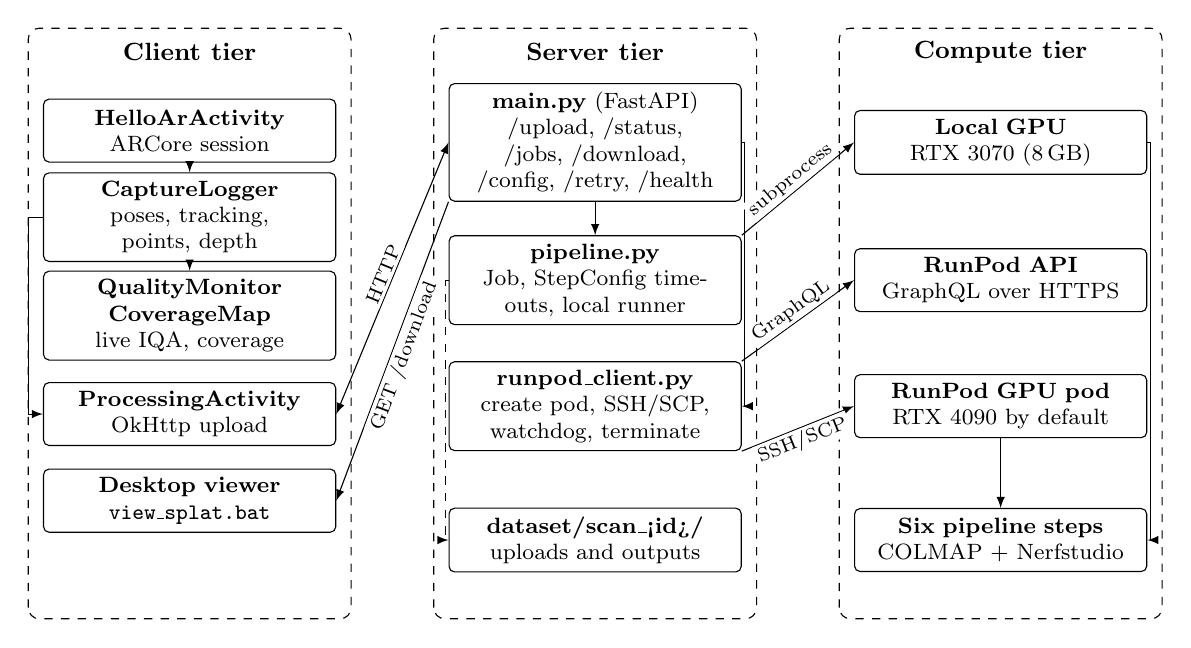
\begin{tikzpicture}[font=\footnotesize, >=latex,
  comp/.style={draw, rectangle, rounded corners=2pt, fill=white, align=center, text width=3.5cm, inner sep=3pt, minimum height=0.8cm},
  tier/.style={draw, dashed, rounded corners=4pt},
  lbl/.style={font=\scriptsize, fill=white, inner sep=1pt}]
  % tiers
  \draw[tier] (-7.2,-3.3) rectangle (-3.1,4.2);
  \draw[tier] (-2.05,-3.3) rectangle (2.05,4.2);
  \draw[tier] (3.1,-3.3) rectangle (7.2,4.2);
  \node[font=\small\bfseries] at (-5.15,3.9) {Client tier};
  \node[font=\small\bfseries] at (0,3.9) {Server tier};
  \node[font=\small\bfseries] at (5.15,3.9) {Compute tier};
  % client tier
  \node[comp] (ar)     at (-5.15,2.9)  {\textbf{HelloArActivity}\\ARCore session};
  \node[comp] (log)    at (-5.15,1.8) {\textbf{CaptureLogger}\\poses, tracking, points, depth};
  \node[comp] (iqa)    at (-5.15,0.55)  {\textbf{QualityMonitor}\\\textbf{CoverageMap}\\live IQA, coverage};
  \node[comp] (proc)   at (-5.15,-0.7) {\textbf{ProcessingActivity}\\OkHttp upload};
  \node[comp] (viewer) at (-5.15,-1.8) {\textbf{Desktop viewer}\\\texttt{view\_splat.bat}};
  % server tier
  \node[comp] (api)   at (0,2.75) {\textbf{main.py} (FastAPI)\\/upload, /status, /jobs, /download, /config, /retry, /health};
  \node[comp] (pipe)  at (0,1.0)  {\textbf{pipeline.py}\\Job, StepConfig timeouts, local runner};
  \node[comp] (rp)    at (0,-0.6) {\textbf{runpod\_client.py}\\create pod, SSH/SCP, watchdog, terminate};
  \node[comp] (store) at (0,-2.3) {\textbf{dataset/scan\_<id>/}\\uploads and outputs};
  % compute tier
  \node[comp] (local) at (5.15,2.75) {\textbf{Local GPU}\\RTX 3070 (8\,GB)};
  \node[comp] (rpapi) at (5.15,1.0)  {\textbf{RunPod API}\\GraphQL over HTTPS};
  \node[comp] (pod)   at (5.15,-0.6) {\textbf{RunPod GPU pod}\\RTX 4090 by default};
  \node[comp] (steps) at (5.15,-2.3) {\textbf{Six pipeline steps}\\COLMAP + Nerfstudio};
  % client-side links
  \draw[->] (ar) -- (log);
  \draw[->] (log) -- (iqa);
  \draw[->] (log.west) -- (-7.2,1.8) -- (-7.2,-0.7) -- (proc.west);
  % client <-> server
  \draw[<->] (proc.east) -- node[lbl, sloped, above] {HTTP} (api.west);
  \draw[->] (api.south west) -- node[lbl, sloped, below] {GET /download} (viewer.east);
  % server internals
  \draw[->] (api) -- (pipe);
  \draw[->] (api.east) -- (1.9,2.75) -- (1.9,-0.6) -- (rp.east);
  \draw[->, dashed] (pipe.west) -- (-1.9,1.0) -- (-1.9,-2.3) -- (store.west);
  % server -> compute
  \draw[->] (pipe.north east) -- node[lbl, sloped, above] {subprocess} (local.west);
  \draw[->] (rp.north east) -- node[lbl, sloped, above] {GraphQL} (rpapi.west);
  \draw[->] (rp.south east) -- node[lbl, sloped, below] {SSH/SCP} (pod.west);
  \draw[->] (pod) -- (steps);
  \draw[->] (local.east) -- (7.05,2.75) -- (7.05,-2.3) -- (steps.east);
\end{tikzpicture}
\caption{System architecture. Client: Android app (\texttt{googleARCore/samples/hello\_ar\_java/}) and the desktop viewer. Server: \texttt{server/main.py}, \texttt{pipeline.py}, \texttt{runpod\_client.py}. Compute: the local GPU, or a RunPod pod reached through the RunPod GraphQL API and SSH/SCP. Both compute paths run the same six steps; \texttt{test\_server\_pipeline.py} checks that the two command lists match.}
\label{fig:architecture}
\end{figure}

\section{Architectural Components}
\label{sec:components}

\paragraph{Android App (\texttt{googleARCore/samples/hello\_ar\_java/})}
\begin{itemize}
    \item \texttt{HelloArActivity}: Main AR camera activity with recording controls, settings menu, and quality overlay.
    \item \texttt{CaptureLogger}: Background I/O thread writing poses, tracking, points, quality, depth, and metadata files.
    \item \texttt{QualityMonitor}: Analyzes camera frames for blur, brightness, motion speed, and texture.
    \item \texttt{CoverageMap}: Voxel-based (10\,cm) coverage tracker with 8-azimuth $\times$ 2-elevation direction awareness.
    \item \texttt{CoverageOverlayView}: Renders red/yellow/green dots over the camera view.
    \item \texttt{ProcessingActivity}: Upload + progress UI with OkHttp multipart client.
\end{itemize}

Figure~\ref{fig:androidarch} shows how these classes and screens connect.

\begin{figure}[htbp]
\centering
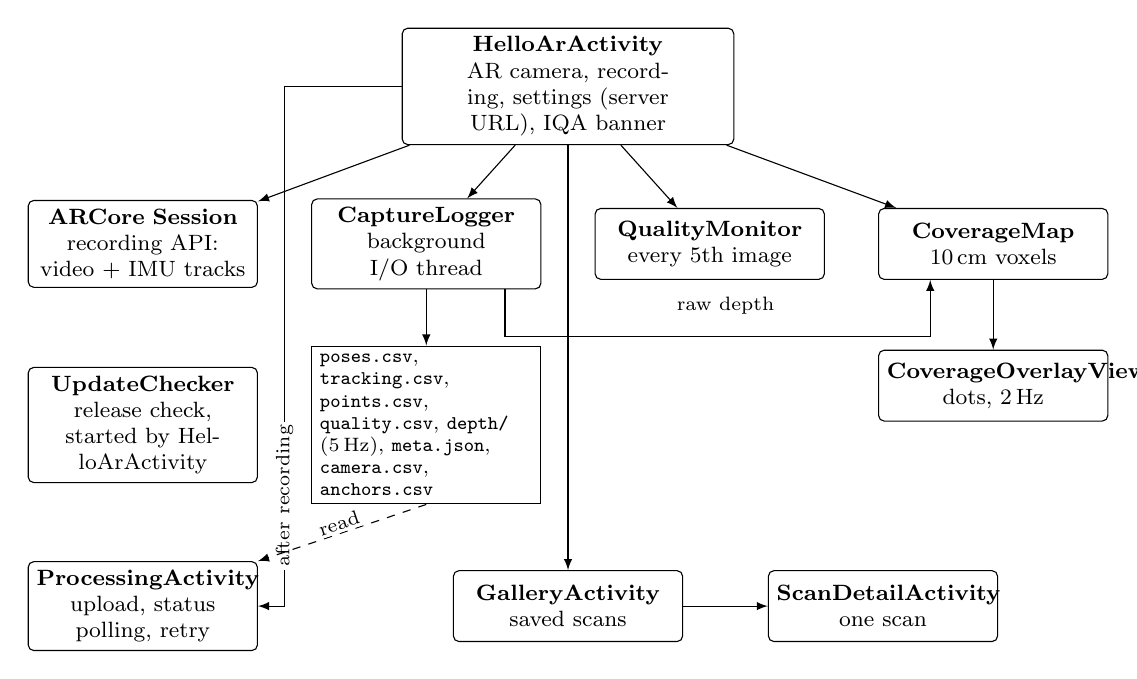
\begin{tikzpicture}[font=\footnotesize, >=latex,
  cls/.style={draw, rectangle, rounded corners=2pt, align=center, text width=2.7cm, inner sep=3pt, minimum height=0.9cm, fill=white},
  lbl/.style={font=\scriptsize, fill=white, inner sep=1pt}]
  \node[cls, text width=4.0cm] (main) at (0,3.2) {\textbf{HelloArActivity}\\AR camera, recording, settings (server URL), IQA banner};
  \node[cls] (sess) at (-5.4,1.2) {\textbf{ARCore Session}\\recording API: video + IMU tracks};
  \node[cls] (log)  at (-1.8,1.2) {\textbf{CaptureLogger}\\background I/O thread};
  \node[cls] (qm)   at (1.8,1.2)  {\textbf{QualityMonitor}\\every 5th image};
  \node[cls] (cov)  at (5.4,1.2)  {\textbf{CoverageMap}\\10\,cm voxels};
  \node[cls] (ov)   at (5.4,-0.6) {\textbf{CoverageOverlayView}\\dots, 2\,Hz};
  \node[draw, rectangle, align=left, text width=2.7cm, inner sep=3pt, font=\scriptsize] (files) at (-1.8,-1.1) {\texttt{poses.csv}, \texttt{tracking.csv}, \texttt{points.csv}, \texttt{quality.csv}, \texttt{depth/} (5\,Hz), \texttt{meta.json}, \texttt{camera.csv}, \texttt{anchors.csv}};
  \node[cls] (upd)  at (-5.4,-1.1) {\textbf{UpdateChecker}\\release check, started by HelloArActivity};
  \node[cls] (proc) at (-5.4,-3.4) {\textbf{ProcessingActivity}\\upload, status polling, retry};
  \node[cls] (gal)  at (0,-3.4)    {\textbf{GalleryActivity}\\saved scans};
  \node[cls] (det)  at (4.0,-3.4)  {\textbf{ScanDetailActivity}\\one scan};
  \draw[->] (main) -- (sess);
  \draw[->] (main) -- (log);
  \draw[->] (main) -- (qm);
  \draw[->] (main) -- (cov);
  \draw[->] (cov) -- (ov);
  \draw[->] ([xshift=1.0cm]log.south) -- ++(0,-0.6) -| ([xshift=-0.8cm]cov.south);
  \node[lbl] at (2.0,0.42) {raw depth};
  \draw[->] (log) -- (files);
  \draw[->] (main.west) -- (-3.6,3.2) -- (-3.6,-3.4) -- (proc.east);
  \node[lbl, rotate=90] at (-3.6,-2.0) {after recording};
  \draw[->] (main.south) -- (gal.north);
  \draw[->] (gal) -- (det);
  \draw[->, dashed] (files.south) -- node[lbl, sloped, above] {read} (proc.north east);
\end{tikzpicture}
\caption{Android capture app (\texttt{googleARCore/samples/hello\_ar\_java/.../helloar/}). Arrows from \texttt{HelloArActivity} show ownership or navigation (\texttt{Intent}s); \texttt{CaptureLogger} feeds raw depth to \texttt{CoverageMap}. \texttt{ProcessingActivity} uploads six files plus a zipped \texttt{depth/} folder; \texttt{camera.csv} and \texttt{anchors.csv} stay on the phone.}
\label{fig:androidarch}
\end{figure}

\paragraph{Processing Server (\texttt{server/})}
\begin{itemize}
    \item \texttt{main.py}: FastAPI endpoints---\texttt{/upload}, \texttt{/status/\{job\_id\}}, \texttt{/jobs}, \texttt{/logs/\{job\_id\}}, \texttt{/retry/\{job\_id\}}, \texttt{/jobs/\{job\_id\}/cancel}, \texttt{/download/\{job\_id\}}, \texttt{/config}, \texttt{/gpus}, \texttt{/datasets}, \texttt{/reprocess}, \texttt{/run-on-pod}, \texttt{/health}.
    \item \texttt{pipeline.py}: Local pipeline runner with \texttt{Job} dataclass, \texttt{StepConfig} per-step timeouts, and subprocess execution with streaming stdout.
    \item \texttt{runpod\_client.py}: RunPod API client (GraphQL pod creation, SSH/SCP helpers, remote pipeline execution, pod watchdog, pod termination in \texttt{finally} blocks).
\end{itemize}

\paragraph{Reconstruction Pipeline (\texttt{src/arcore3dgs/})}
\begin{itemize}
    \item \texttt{fallback.py}: IMU-bridged tracking-gap recovery.
    \item \texttt{prepare.py}: Keyframe extraction from video (sharpest frame by Laplacian variance in each window of 8 frames).
    \item \texttt{select\_sharp.py}: Gyro-aware keyframe selection (least predicted motion blur per 0.2\,s window). Used for the v4--v6 models; not yet part of the one-command pipeline.
    \item \texttt{sfm\_colmap.py}: COLMAP SIFT matching + global mapper + lens self-calibration + Sim3 alignment to ARCore metric frame.
    \item \texttt{export\_nerfstudio.py}: Convert COLMAP output to Nerfstudio data format.
    \item Nerfstudio \texttt{ns-train splatfacto}: 3DGS training (30k iterations).
    \item Nerfstudio \texttt{ns-export}: Export \texttt{splat.ply}.
\end{itemize}

\section{Interfaces and Dependencies}

\begin{table}[htbp]
\centering
\small
\caption{Key interfaces between components}
\label{tab:interfaces}
\begin{tabular}{p{3cm}p{3cm}p{5cm}}
\toprule
\textbf{From} & \textbf{To} & \textbf{Interface} \\
\midrule
Android App & Server & HTTP multipart POST (\texttt{/upload}) \\
Android App & Server & HTTP GET polling (\texttt{/status/\{id\}}) \\
Server & RunPod API & GraphQL over HTTPS \\
Server & GPU Pod & SSH/SCP over TCP \\
Pipeline steps & Next step & Filesystem (dataset directory) \\
\texttt{sfm\_colmap.py} & splatfacto & \texttt{transforms.json} + images \\
\bottomrule
\end{tabular}
\end{table}

\paragraph{External dependencies:} Google ARCore SDK (Android), COLMAP 4.2 (SfM/MVS), Nerfstudio 1.1.5 (3DGS training), OkHttp 4.12.0 (Android HTTP client), FastAPI + Uvicorn (Python web framework) and the RunPod API (cloud GPU provisioning).

\section{Architecture Decisions and Rationale}

\begin{enumerate}
    \item \textbf{COLMAP SfM over ARCore poses for training}: Raw ARCore poses have a 2.32\,px median reprojection error (slow drift); bundle adjustment reduces this to 0.62\,px, but ARCore also re-anchors silently (every pose before $\sim$60\,s was off by $\sim$1\,m and 28\textdegree) and reports no lens distortion. COLMAP's SfM with self-calibrated lens distortion ($k_1 \approx 0.09$, $k_2 \approx -0.22$) removes both. On the same recording, training-view fit rose from 21.9\,dB to $\sim$28\,dB, held-out SSIM from 0.78 to 0.86, and badly placed surfaces fell from 7--23\% to 3\%.

    \item \textbf{Splatfacto over custom trainer}: After extensive analysis showing our custom training recipe produced degenerate splats, we adopted Nerfstudio's battle-tested splatfacto implementation. On a separate scene (\texttt{roomAttemptSadness2}), splatfacto reached 27.81\,dB held-out against 24.70\,dB for our corrected custom trainer on the same inputs. Our value-add is in the preprocessing (ARCore integration, metric alignment, IMU fallback, quality guidance).

    \item \textbf{RunPod on-demand over serverless}: On-demand pods allow full SSH control of the pipeline, suit long-running jobs (about 75\,min end-to-end measured on an RTX 3070), and support arbitrary software installation. Serverless endpoints have cold-start latency and timeout limits that conflict with COLMAP's variable runtime.

    \item \textbf{HTTP polling over WebSockets}: Simpler implementation, works across firewalls/proxies, and 3-second polling interval is sufficient for a pipeline that takes minutes.
\end{enumerate}

\section{Design Evolution}
\begin{enumerate}
    \item \textbf{Proposal $\rightarrow$ Mid}: Added live IQA and coverage guidance (not in original proposal). Changed from ARCore-pose-based training to COLMAP SfM-based training after discovering ARCore's pose accuracy limitations. On the way, the team's own GPU bundle adjustment, Metric3D depth, own stereo matcher, depth supervision, floater pruning, median filtering and post-hoc flat-forcing were tried and parked (Section~\ref{sec:parked}).

    \item \textbf{Custom trainer $\rightarrow$ splatfacto}: After two weeks of analysis documenting six root causes of degenerate splat geometry, we switched training to Nerfstudio splatfacto. The custom preprocessing pipeline was retained and validated.

    \item \textbf{Local-only $\rightarrow$ local + cloud}: Added RunPod cloud GPU support to enable processing on machines without a GPU, and to support faster GPUs (RTX 4090 by default) than the development machine (RTX 3070, 8\,GB).
\end{enumerate}

\section{Domain Model}
The core domain entities are:
\begin{itemize}
    \item \textbf{Scan}: A recording session producing a dataset (video + sensor files).
    \item \textbf{Dataset}: The collection of files from one scan (video, poses, depth, quality, meta).
    \item \textbf{Job}: A processing task with status (queued, processing, completed, failed), progress, and output path. Its life cycle is shown in Figure~\ref{fig:jobstate}.
    \item \textbf{Model}: The output 3D Gaussian Splatting model (\texttt{splat.ply}).
    \item \textbf{Measurement}: A point-to-point distance in the metric model (FYP-2).
\end{itemize}

\begin{figure}[htbp]
\centering
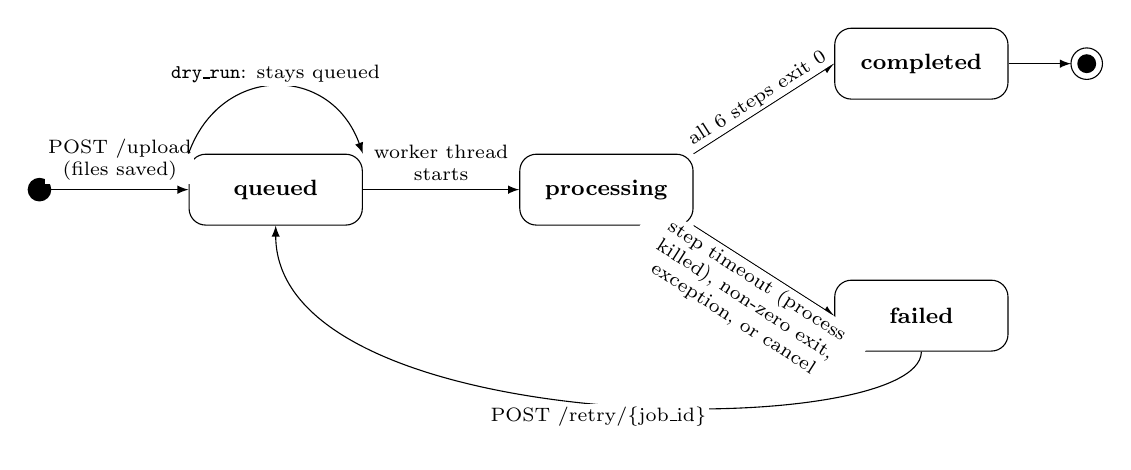
\begin{tikzpicture}[font=\footnotesize, >=latex,
  state/.style={draw, rectangle, rounded corners=6pt, minimum width=2.2cm, minimum height=0.9cm, align=center},
  lbl/.style={font=\scriptsize, align=center, fill=white, inner sep=1pt}]
  \fill (-6.6,0) circle (0.15);
  \node[state] (queued) at (-3.6,0) {\textbf{queued}};
  \node[state] (proc)   at (0.6,0)  {\textbf{processing}};
  \node[state] (done)   at (4.6,1.6) {\textbf{completed}};
  \node[state] (failed) at (4.6,-1.6) {\textbf{failed}};
  \draw (6.7,1.6) circle (0.2);
  \fill (6.7,1.6) circle (0.12);
  \draw[->] (-6.45,0) -- node[lbl, above=2pt] {POST /upload\\(files saved)} (queued.west);
  \draw[->] (queued.east) -- node[lbl, above=2pt] {worker thread\\starts} (proc.west);
  \draw[->] (queued.north west) .. controls (-4.3,1.6) and (-2.9,1.6) .. node[lbl, above] {\texttt{dry\_run}: stays queued} (queued.north east);
  \draw[->] (proc.north east) -- node[lbl, sloped, above] {all 6 steps exit 0} (done.west);
  \draw[->] (proc.south east) -- node[lbl, sloped, below, text width=3.2cm] {step timeout (process killed), non-zero exit, exception, or cancel} (failed.west);
  \draw[->] (done.east) -- (6.5,1.6);
  \draw[->] (failed.south) .. controls (4.6,-3.2) and (-3.6,-3.2) .. node[lbl, below] {POST /retry/\{job\_id\}} (queued.south);
\end{tikzpicture}
\caption{Job state machine (\texttt{JobStatus} in \texttt{server/pipeline.py}). A timeout is enforced per step by the watchdog loop in \texttt{run\_pipeline()}, which kills the subprocess and marks the job failed; cancel is \texttt{POST /jobs/\{job\_id\}/cancel}. In RunPod mode a separate pod watchdog terminates the pod after \texttt{MAX\_POD\_LIFETIME} (default 7200\,s). An \texttt{uploading} value is defined in \texttt{JobStatus} but no code path sets it.}
\label{fig:jobstate}
\end{figure}

\section{Data Design}

\paragraph{Capture data (per scan):}
\begin{itemize}
    \item \texttt{dataset.mp4}: H.264 video, 1920$\times$1080, 30\,FPS.
    \item \texttt{poses.csv}: timestamp, tx, ty, tz, qx, qy, qz, qw, fx, fy, cx, cy (per frame).
    \item \texttt{tracking.csv}: timestamp, tracking\_state, failure\_reason (per frame).
    \item \texttt{points.csv}: timestamp, point\_id, x, y, z, confidence (ARCore feature points).
    \item \texttt{quality.csv}: timestamp, sharpness, brightness, motion\_speed, texture\_level (per analyzed frame).
    \item \texttt{depth/}: uint16 depth maps (mm) + uint8 confidence maps at 5\,Hz.
    \item \texttt{meta.json}: device model, camera config, resolution, ARCore version.
\end{itemize}

\paragraph{Pipeline intermediate data:}
\begin{itemize}
    \item \texttt{poses\_fused.csv}, \texttt{fallback\_report.json}: poses with tracking gaps bridged by the IMU.
    \item \texttt{work/images/}, \texttt{work/frames.json}: extracted keyframes (JPEG) and their ARCore poses.
    \item \texttt{work\_sfm/}: COLMAP database, sparse model, undistorted images, Sim3-aligned \texttt{frames.json}, \texttt{init\_points.ply}.
    \item \texttt{work\_sfm/transforms.json}: Nerfstudio-format camera transforms.
    \item \texttt{work\_sfm/gs\_sfm/splat.ply}: Final 3DGS model.
\end{itemize}

Figure~\ref{fig:dataflow} traces the capture files through the six pipeline steps. \texttt{quality.csv}, \texttt{meta.json} and \texttt{depth/} are uploaded and stored with the dataset, but the current six steps do not read them (keyframe extraction runs with \texttt{--depth 0}).

\begin{figure}[htbp]
\centering
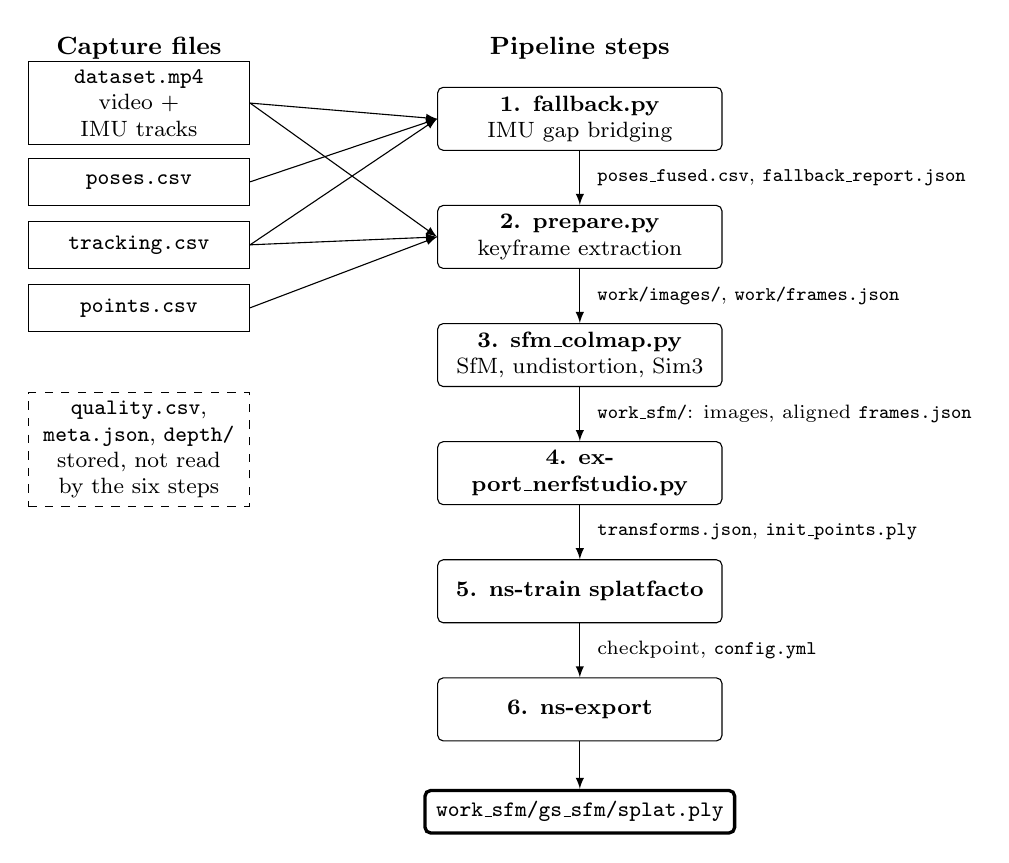
\begin{tikzpicture}[font=\footnotesize, >=latex,
  file/.style={draw, rectangle, align=center, text width=2.6cm, inner sep=3pt, minimum height=0.6cm},
  pstep/.style={draw, rectangle, rounded corners=2pt, align=center, text width=3.4cm, inner sep=3pt, minimum height=0.8cm, fill=white},
  lbl/.style={font=\scriptsize, anchor=west}]
  % capture files
  \node[font=\small\bfseries] at (-5.2,3.5) {Capture files};
  \node[file] (mp4)  at (-5.2,2.8)  {\texttt{dataset.mp4}\\video + IMU tracks};
  \node[file] (pose) at (-5.2,1.8)  {\texttt{poses.csv}};
  \node[file] (trk)  at (-5.2,1.0)  {\texttt{tracking.csv}};
  \node[file] (pts)  at (-5.2,0.2)  {\texttt{points.csv}};
  \node[file, dashed] (unused) at (-5.2,-1.6) {\texttt{quality.csv}, \texttt{meta.json}, \texttt{depth/}\\stored, not read by the six steps};
  % steps
  \node[font=\small\bfseries] at (0.4,3.5) {Pipeline steps};
  \node[pstep] (s1) at (0.4,2.6)  {\textbf{1. fallback.py}\\IMU gap bridging};
  \node[pstep] (s2) at (0.4,1.1)  {\textbf{2. prepare.py}\\keyframe extraction};
  \node[pstep] (s3) at (0.4,-0.4) {\textbf{3. sfm\_colmap.py}\\SfM, undistortion, Sim3};
  \node[pstep] (s4) at (0.4,-1.9) {\textbf{4. export\_nerfstudio.py}};
  \node[pstep] (s5) at (0.4,-3.4) {\textbf{5. ns-train splatfacto}};
  \node[pstep] (s6) at (0.4,-4.9) {\textbf{6. ns-export}};
  \node[draw, very thick, rectangle, rounded corners=2pt, inner sep=4pt] (out) at (0.4,-6.2) {\texttt{work\_sfm/gs\_sfm/splat.ply}};
  % inputs
  \draw[->] (mp4.east)  -- (s1.west);
  \draw[->] (pose.east) -- (s1.west);
  \draw[->] (trk.east)  -- (s1.west);
  \draw[->] (mp4.east)  -- (s2.west);
  \draw[->] (trk.east)  -- (s2.west);
  \draw[->] (pts.east)  -- (s2.west);
  % chain
  \draw[->] (s1) -- (s2);
  \node[lbl] at (0.5,1.85) {\texttt{poses\_fused.csv}, \texttt{fallback\_report.json}};
  \draw[->] (s2) -- (s3);
  \node[lbl] at (0.5,0.35) {\texttt{work/images/}, \texttt{work/frames.json}};
  \draw[->] (s3) -- (s4);
  \node[lbl] at (0.5,-1.15) {\texttt{work\_sfm/}: images, aligned \texttt{frames.json}};
  \draw[->] (s4) -- (s5);
  \node[lbl] at (0.5,-2.65) {\texttt{transforms.json}, \texttt{init\_points.ply}};
  \draw[->] (s5) -- (s6);
  \node[lbl] at (0.5,-4.15) {checkpoint, \texttt{config.yml}};
  \draw[->] (s6) -- (out);
\end{tikzpicture}
\caption{Data flow from the capture files to the model, as run by \texttt{server/pipeline.py} (and, step for step, on a RunPod pod). Steps 1--2 read the capture through \texttt{common.Capture}; \texttt{fallback.py} reads the IMU samples from the MP4's own data tracks (\texttt{imu.py}).}
\label{fig:dataflow}
\end{figure}

\section{Process / Behavior Design}
\label{sec:process}

The end-to-end pipeline follows a sequential six-step process:

\begin{enumerate}
    \item \textbf{Fallback} (2\,min timeout): Read the gyroscope and accelerometer samples stored in \texttt{dataset.mp4}, find tracking gaps in \texttt{tracking.csv}, and bridge them with IMU integration anchored at both ends of each gap.
    \item \textbf{Prepare} (5\,min timeout): Decode video, keep the sharpest frame (Laplacian variance) in each window of 8 frames, extract to JPEG (\texttt{prepare.py}). The gyro-aware selection of \texttt{select\_sharp.py} that produced v6 is not yet in this step.
    \item \textbf{SfM} (40\,min timeout): COLMAP feature extraction (SIFT), exhaustive matching, global mapper, lens self-calibration, image undistortion, Sim3 alignment to ARCore metric frame.
    \item \textbf{Export} (2\,min timeout): Convert COLMAP output to Nerfstudio \texttt{transforms.json} format.
    \item \textbf{Train} (60\,min timeout): Nerfstudio splatfacto training (30k iterations) with bilateral grid exposure compensation, scale regularization, and fixed poses.
    \item \textbf{Export Model} (5\,min timeout): Export trained model to \texttt{splat.ply}.
\end{enumerate}

Figure~\ref{fig:pipelinesteps} shows the steps with their timeouts and the measured times.

\begin{figure}[htbp]
\centering
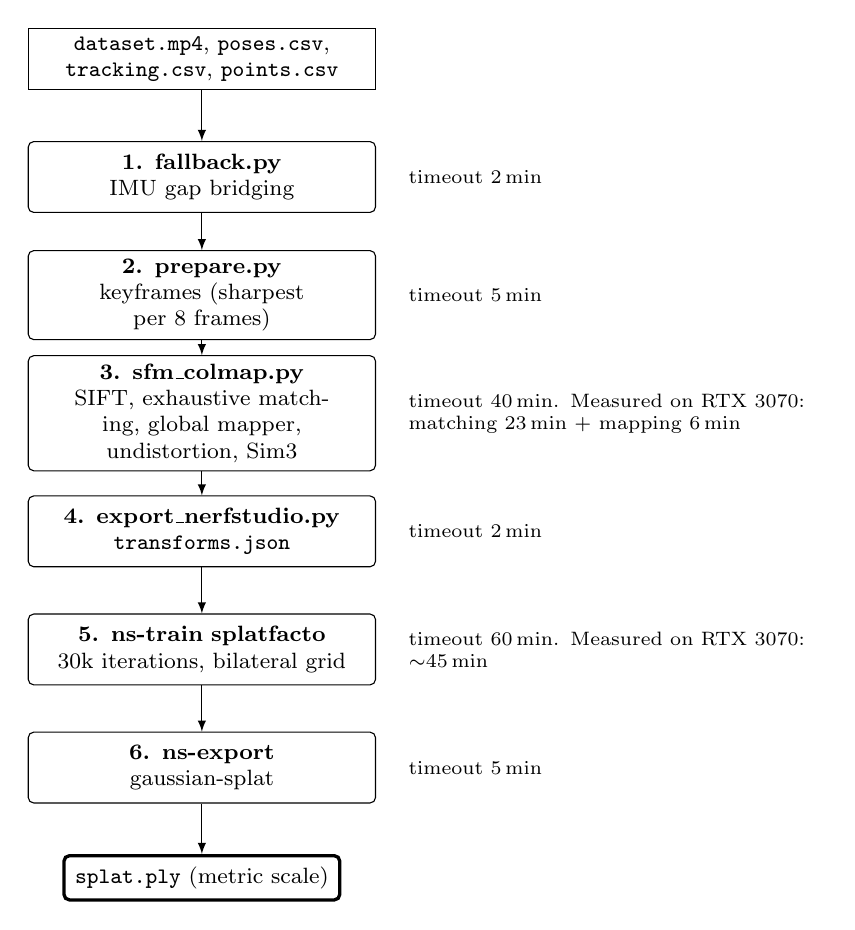
\begin{tikzpicture}[font=\footnotesize, >=latex,
  pstep/.style={draw, rectangle, rounded corners=2pt, align=center, text width=4.2cm, inner sep=3pt, minimum height=0.9cm},
  note/.style={font=\scriptsize, anchor=west, align=left, text width=5.2cm}]
  \node[draw, rectangle, align=center, text width=4.2cm, inner sep=3pt] (in) at (-2.4,1.5) {\texttt{dataset.mp4}, \texttt{poses.csv}, \texttt{tracking.csv}, \texttt{points.csv}};
  \node[pstep] (s1) at (-2.4,0)    {\textbf{1. fallback.py}\\IMU gap bridging};
  \node[pstep] (s2) at (-2.4,-1.5) {\textbf{2. prepare.py}\\keyframes (sharpest per 8 frames)};
  \node[pstep] (s3) at (-2.4,-3.0) {\textbf{3. sfm\_colmap.py}\\SIFT, exhaustive matching, global mapper, undistortion, Sim3};
  \node[pstep] (s4) at (-2.4,-4.5) {\textbf{4. export\_nerfstudio.py}\\\texttt{transforms.json}};
  \node[pstep] (s5) at (-2.4,-6.0) {\textbf{5. ns-train splatfacto}\\30k iterations, bilateral grid};
  \node[pstep] (s6) at (-2.4,-7.5) {\textbf{6. ns-export}\\gaussian-splat};
  \node[draw, very thick, rectangle, rounded corners=2pt, inner sep=4pt] (out) at (-2.4,-8.9) {\texttt{splat.ply} (metric scale)};
  \draw[->] (in) -- (s1);
  \draw[->] (s1) -- (s2);
  \draw[->] (s2) -- (s3);
  \draw[->] (s3) -- (s4);
  \draw[->] (s4) -- (s5);
  \draw[->] (s5) -- (s6);
  \draw[->] (s6) -- (out);
  \node[note] at (0.1,0)    {timeout 2\,min};
  \node[note] at (0.1,-1.5) {timeout 5\,min};
  \node[note] at (0.1,-3.0) {timeout 40\,min. Measured on RTX 3070: matching 23\,min + mapping 6\,min};
  \node[note] at (0.1,-4.5) {timeout 2\,min};
  \node[note] at (0.1,-6.0) {timeout 60\,min. Measured on RTX 3070: $\sim$45\,min};
  \node[note] at (0.1,-7.5) {timeout 5\,min};
\end{tikzpicture}
\caption{The six pipeline steps and their timeouts (\texttt{STEPS} in \texttt{server/pipeline.py}). The measured end-to-end time on the development RTX 3070 is $\sim$75\,min; no cloud-GPU time has been measured yet.}
\label{fig:pipelinesteps}
\end{figure}

Each step is executed as a subprocess with streaming stdout captured for progress reporting. If a step exceeds its timeout, the process is killed and the job is marked failed. In RunPod mode, whenever a pod has been created it is terminated in a \texttt{finally} block regardless of success or failure, and a watchdog thread terminates it after \texttt{MAX\_POD\_LIFETIME} (default 7200\,s). Figure~\ref{fig:sequence} shows the upload $\rightarrow$ process $\rightarrow$ download interaction in RunPod mode.

\begin{figure}[p]
\centering
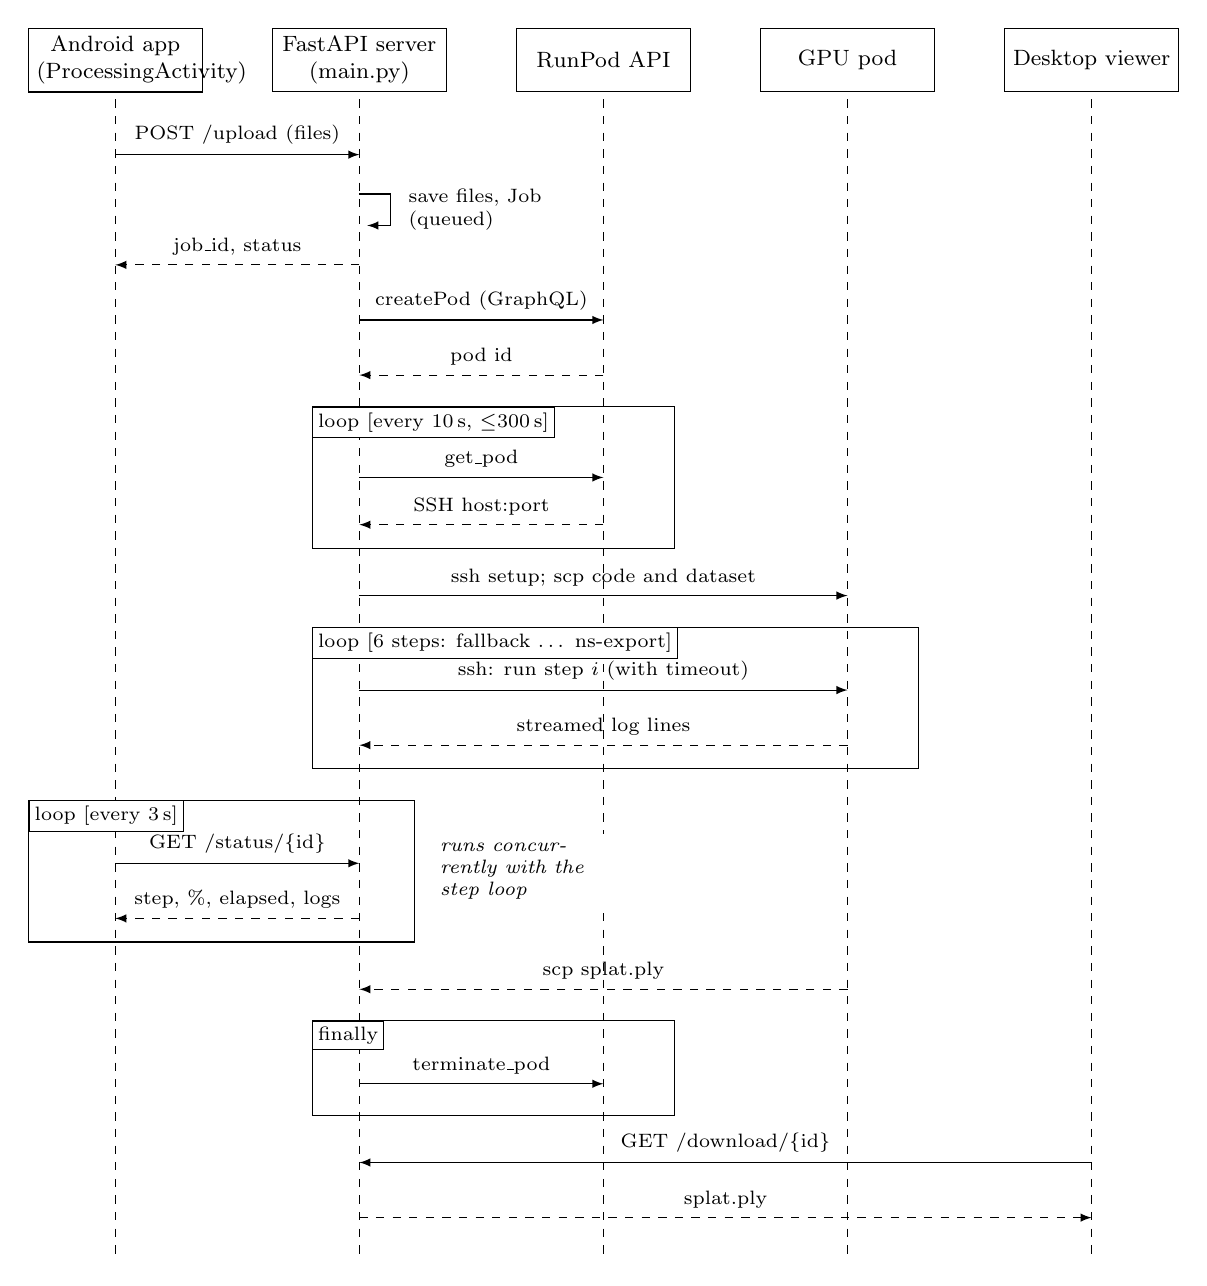
\begin{tikzpicture}[font=\footnotesize, >=latex,
  head/.style={draw, rectangle, align=center, text width=2.0cm, inner sep=3pt, minimum height=0.8cm, fill=white},
  msg/.style={font=\scriptsize, above, align=center},
  frame/.style={draw, rectangle},
  tab/.style={draw, fill=white, font=\scriptsize, anchor=north west, inner sep=2pt}]
  % lifelines
  \foreach \x/\lab in {-6.2/{Android app\\(ProcessingActivity)}, -3.1/{FastAPI server\\(main.py)}, 0/{RunPod API}, 3.1/{GPU pod}, 6.2/{Desktop viewer}} {
    \draw[dashed] (\x,-0.5) -- (\x,-15.2);
    \node[head] at (\x,0) {\lab};
  }
  % upload
  \draw[->] (-6.2,-1.2) -- node[msg] {POST /upload (files)} (-3.1,-1.2);
  \draw[->] (-3.1,-1.7) -- (-2.7,-1.7) -- (-2.7,-2.1) -- (-3.0,-2.1);
  \node[font=\scriptsize, anchor=west, text width=2.4cm] at (-2.6,-1.9) {save files, Job (queued)};
  \draw[->, dashed] (-3.1,-2.6) -- node[msg] {job\_id, status} (-6.2,-2.6);
  % pod creation
  \draw[->] (-3.1,-3.3) -- node[msg] {createPod (GraphQL)} (0,-3.3);
  \draw[->, dashed] (0,-4.0) -- node[msg] {pod id} (-3.1,-4.0);
  \draw[frame] (-3.7,-4.4) rectangle (0.9,-6.2);
  \node[tab] at (-3.7,-4.4) {loop [every 10\,s, $\leq$300\,s]};
  \draw[->] (-3.1,-5.3) -- node[msg] {get\_pod} (0,-5.3);
  \draw[->, dashed] (0,-5.9) -- node[msg] {SSH host:port} (-3.1,-5.9);
  \draw[->] (-3.1,-6.8) -- node[msg] {ssh setup; scp code and dataset} (3.1,-6.8);
  % pipeline steps
  \draw[frame] (-3.7,-7.2) rectangle (4.0,-9.0);
  \node[tab] at (-3.7,-7.2) {loop [6 steps: fallback \ldots\ ns-export]};
  \draw[->] (-3.1,-8.0) -- node[msg] {ssh: run step $i$ (with timeout)} (3.1,-8.0);
  \draw[->, dashed] (3.1,-8.7) -- node[msg] {streamed log lines} (-3.1,-8.7);
  % polling
  \draw[frame] (-7.3,-9.4) rectangle (-2.4,-11.2);
  \node[tab] at (-7.3,-9.4) {loop [every 3\,s]};
  \draw[->] (-6.2,-10.2) -- node[msg] {GET /status/\{id\}} (-3.1,-10.2);
  \draw[->, dashed] (-3.1,-10.9) -- node[msg] {step, \%, elapsed, logs} (-6.2,-10.9);
  \node[font=\scriptsize\itshape, anchor=west, text width=2.2cm, fill=white] at (-2.2,-10.3) {runs concurrently with the step loop};
  \draw[->, dashed] (3.1,-11.8) -- node[msg] {scp splat.ply} (-3.1,-11.8);
  % termination
  \draw[frame] (-3.7,-12.2) rectangle (0.9,-13.4);
  \node[tab] at (-3.7,-12.2) {finally};
  \draw[->] (-3.1,-13.0) -- node[msg] {terminate\_pod} (0,-13.0);
  % download
  \draw[->] (6.2,-14.0) -- node[msg] {GET /download/\{id\}} (-3.1,-14.0);
  \draw[->, dashed] (-3.1,-14.7) -- node[msg] {splat.ply} (6.2,-14.7);
\end{tikzpicture}
\caption{Sequence diagram for upload $\rightarrow$ process $\rightarrow$ download in RunPod mode (\texttt{ProcessingActivity.java}, \texttt{server/main.py}, \texttt{run\_pipeline\_on\_runpod()} in \texttt{server/runpod\_client.py}). The app polls every 3\,s (5\,s after an error) and stops when the status is \texttt{completed} or \texttt{failed}. The app does not download the model; it is fetched with \texttt{GET /download} by the desktop viewer.}
\label{fig:sequence}
\end{figure}
